CPU-Rechenzeit ist eine wertvolle Ressource und muss finanziert werden. Weiterhin erfreut es den (zumeist ungeduldigen) Anwender, wenn das Ergebnis einer quantenchemischen Rechnung möglichst schnell erhalten wird. Aus diesem Grund ist die Effizienzsteigerung immer ein aktuelles Forschungsgebiet. Eine Möglichkeit, Rechnungen effizienter durchzuführen ist durch das Einführen von Näherungen gegeben. Jedoch darf die Genauigkeit des Resultats nicht unter diesen Näherungsmethoden leiden. Eine weit gebräuchliche Näherung ist die \aclu*{ri-}\mbox{(\acs{ri}-)}\acused{ri}Näherung\supercite{vahtras1993integral}, deren Idee ursprünglich auf Dunlap\supercite{dunlap1979some} und Whitten\supercite{whitten1973coulombic} zurückzuführen ist. Der Einsatz dieser Methode bei der Berechnung von chemischen Abschirmungskonstanten sowie eine weitere Beschleunigung durch die Verwendung einer Multipolentwicklung sind in den folgenden Abschnitten \ref{ri} und \ref{marij} erläutert. Effizienzsteigerungen und Genauigkeitseinbußen werden in Kapitel \ref{genauigkeit} untersucht. Optimierungen des Programmcodes und effizientes Abschätzen verschwindender Integralbeiträge stellen weitere Möglichkeiten dar, um die Effizienz zu verbessern. Zusätzlich führt die Parallelisierung des Programmcodes zu einer verkürzten Laufzeit der Berechnungen. Diese letztgenannten Punkte sind in Abschnitt \ref{paraopt} zusammengefasst. 
Mithilfe dieser Methoden soll im Rahmen der vorliegenden Arbeit die Möglichkeit geschaffen werden, \ac{nmr}-Abschirmungskonstanten und die magnetische Response für große Moleküle mit mehreren tausend Atomen berechnen zu können.  

\section{Die RI-Methode für chemische Abschirmungskonstanten}\label{ri}
Die \aclu*{ri-}\mbox{(\acs{ri}-)}\acused{ri}Näherung stellt in der \ac{scf}-Prozedur ein bewährtes Näherungsverfahren zur Berechnung der Vierzentren-Zweielektronen-Integrale dar. Diese setzen sich aus dem Coulombterm und dem Austauschterm zusammen, und ihre Berechnung ist der zeitaufwändigste Schritt während des Verfahrens. Insbesondere der Coulombterm lässt sich durch das Anwenden der \ac{ri}-Näherung deutlich effizienter berechnen. Dies gilt bereits für kleine Basissätze von \textit{double}-$\zeta$-Qualität und wird für größere Basissätze noch effizienter. Prinzipiell kann die Näherung auch für den Austauschterm angewendet werden, die Rechenzeiten verkürzen sich jedoch erst deutlich bei größeren Basissätzen ab \textit{quadruple}-$\zeta$-Qualität. Wird nur der Coulombterm oder nur der Austauschbeitrag angenähert, so wird von \ac{ri}-\textit{J} oder \ac{ri}-\textit{K} gesprochen, bzw. \ac{ri}-\textit{JK}, wenn die Näherung für beide Terme angewendet wird. 

Auch bei der Berechnung chemischer Abschirmungskonstanten ist die Auswertung der abgeleiteten Zweielektronen-Integrale zeitbestimmend. Dies gilt insbesondere dann, wenn reine Dichtefunktionale (d.\,h. keine Hybridfunktionale mit Hartree-Fock-Austausch) verwendet werden, da für sie im Rahmen der \textit{uncoupled}-\ac{dft} keine \ac{cphf}-Gleichungen gelöst werden müssen. Die \ac{ri}-Näherung lässt sich auch auf die abgeleiteten Zweielektronen-Integrale übertragen, wobei die Näherung in dieser Arbeit lediglich auf den abgeleiteten Coulombterm übertragen wird. Die Gleichungen für eine mögliche Implementierung des \acs{rik}-Verfahrens sind im Anhang gegeben. Das getrennte Berechnen der Coulomb- und Austauschterme hat weiterhin den Vorteil, dass für die konventionelle Berechnung des Austauschbeitrages eine effizientere Integralabschätzung angewendet werden kann. Dies ist durch die mit dem Abstand schneller abfallende Austauschwechselwirkung begründet. Weiteres dazu wird in Abschnitt \ref{paraopt} erläutert. 
	\subsection{Theorie}
	An dieser Stelle sollen zunächst die grundlegende Idee der Näherung und die daraus resultierenden Formeln aus Referenz \cite{vahtras1993integral} wiedergegeben werden. Im Anschluss daran folgt die Übertragung auf die nach den Komponenten des Magnetfeldes abgeleiteten Coulombintegrale. 
	
	Die Berechnung der Coulombintegrale skaliert formell mit der Anzahl der Basisfunktionen $N_\textrm{BF}$ wie $\mathcal{O}(N_\textrm{BF}^4)$. Durch Anwenden der \ac{ri}-Näherung lässt sich das formelle Skalierungsverhalten um eine Potenz erniedrigen. Die Vierzentren-Integrale lassen sich als Summe des Produkts von Zwei- und Dreizentren-Integralen schreiben, welche wie $\mathcal{O}(N_\textrm{BF}^2)$ und $\mathcal{O}(N_\textrm{BF}^3)$ skalieren. Um dies zu erreichen, wird das Produkt zweier Basisfunktionen $\chi_\mu$ und $\chi_\nu$ durch die Linearkombination von sogenannten atomzentrierten Auxiliarbasisfunktionen $P$ angenähert	
	\begin{equation}
	\gamma_{\mu\nu}=\chi_\mu\chi_\nu\approx\sum_PC^P_{\mu\nu}P=\tilde{\gamma}_{\mu\nu}\, .
	\end{equation}
	
	Durch die Minimierung des Fehlers
	\begin{equation}
	\Delta\gamma_{\mu\nu} = \gamma_{\mu\nu}-\tilde{\gamma}_{\mu\nu}
	\end{equation}
	
	wird letztendlich ein genäherter Ausdruck für die Vierzentren-Integrale erhalten	
	\begin{equation}\label{eq:munukalari}
	\left(\chi_\mu\chi_\nu\vert\chi_\kappa\chi_\lambda\right)\approx\sum_{PQ}^{N_{\textrm{AuxBF}}}\left(\chi_\mu\chi_\nu\right.\underbrace{\left.\vert P\right)\left(P\vert Q\right)^{-1}\left(Q\vert\right.}_{\approx 1}\left.\chi_\kappa\chi_\lambda\right).		
	\end{equation}
	Mit dem Ausdruck oberhalb der geschweiften Klammer in Gleichung (\ref{eq:munukalari}) wird formell eine -- der Methode namensgebende -- Zerlegung der Einheit (englisch \acf{ri}) eingeführt.
	Für eine effiziente Berechnung der Coulombmatrixelemente $J_{\mu\nu}$, wofür Gleichung (\ref{eq:munukalari}) noch mit der Dichtematrix $D_{\kappa\lambda}$ kontrahiert werden muss, wird zunächst die inverse $\left(P\vert Q\right)^{-1}$-Matrix gebildet und mit den Dreizentren-Integralen $\left(Q\vert\chi_\kappa\chi_\lambda\right)$ sowie der Dichtematrix zur intermediären Größe $\Gamma_P$ verarbeitet,
	\begin{equation}
	\Gamma_P=\sum_Q^{N_{\textrm{AuxBF}}}\left(P\vert Q\right)^{-1}\underbrace{\sum_{\kappa\lambda}D_{\kappa\lambda}\left(Q\vert\chi_\kappa\chi_\lambda\right)}_{\Gamma_Q}.
	\end{equation}
	
	Die eigentliche Berechnung von $J_{\mu\nu}$ erfolgt durch Kontrahieren der Dreizentren-Integrale $\left(\chi_\mu\chi_\nu\vert P\right)$ mit $\Gamma_P$,
	\begin{equation}
	J_{\mu\nu}=\sum_{\kappa\lambda}D_{\kappa\lambda}\left(\chi_\mu\chi_\nu\vert\chi_\kappa\chi_\lambda\right)\approx\sum_{P}^{N_{\textrm{AuxBF}}}\left(\chi_\mu\chi_\nu\vert P\right)\Gamma_P=J_{\mu\nu}^{\textrm{RI}}\, .
	\end{equation}
	
	Bei sorgfältig gewählten Auxiliarbasisfunktionen $P$ sind die Fehler, die durch diese Näherung gemacht werden, klein und von wenig Bedeutung\supercite{eichkorn1995auxiliary} im Vergleich zu den Fehlern der Methoden an sich. Die \ac{ri}-Näherung lässt sich nun auch auf den nach den Komponenten des Magnetfeldes abgeleiteten Coulombterm übertragen. Wie bereits zuvor erwähnt, gilt
	\begin{equation}\label{eq:jmunudb}
	\begin{aligned}
	J_{\mu\nu}^{B_\beta}=&\frac{\partial}{\partial B_\beta}\left(\sum_{\kappa\lambda}D_{\kappa\lambda}\left(\chi_\mu\chi_\nu\vert\chi_\kappa\chi_\lambda\right)\right)_{\vec{B}=0}\\
	=&\sum_{\kappa\lambda}\left[D_{\kappa\lambda}^{B_\beta}\left(\chi_\mu^{\vec{B}=0}\chi_\nu^{\vec{B}=0}\vert\chi_\kappa^{\vec{B}=0}\chi_\lambda^{\vec{B}=0}\right)+D_{\kappa\lambda}\left(\overline{\chi_\mu\chi_\nu}\vert\chi_\kappa^{\vec{B}=0}\chi_\lambda^{\vec{B}=0}\right)_{\beta}\right.\\
    &+\left.D_{\kappa\lambda}\left(\chi_\mu^{\vec{B}=0}\chi_\nu^{\vec{B}=0}\vert\overline{\chi_\kappa\chi_\lambda}\right)_{\beta}\right]\\
    =&\sum_{\kappa\lambda}D_{\kappa\lambda}\left(\overline{\chi_\mu\chi_\nu}\vert\chi_\kappa^{\vec{B}=0}\chi_\lambda^{\vec{B}=0}\right)_{\beta}\, ,
	\end{aligned}
	\end{equation}
	da bei den verschwindenden Termen in Gleichung (\ref{eq:jmunudb}) jeweils die Spur des Produkts einer symmetrischen Matrix mit einer antisymmetrischen Matrix gebildet wird. Es muss folglich nur die linke Seite des Integrals, also nur das Produkt der Basisfunktionen $\chi_\mu$ und $\chi_\nu$, abgeleitet werden. Das Einsetzen der \ac{ri}-Näherung liefert daher
	\begin{equation}\label{eq:jmunudbri}
	\begin{aligned}
	J_{\mu\nu}^{B_\beta}\approx &\sum_{PQ}^{N_{\textrm{AuxBF}}}\left(\overline{\chi_\mu\chi_\nu}\vert P\right)_\beta\left(P\vert Q\right)^{-1}\sum_{\kappa\lambda}D_{\kappa\lambda}\left(Q\left\vert\chi_\kappa^{\vec{B}=0}\chi_\lambda^{\vec{B}=0}\right.\right)\\
	=&\sum_{P}^{N_{\textrm{AuxBF}}}\left(\overline{\chi_\mu\chi_\nu}\vert P\right)_\beta\Gamma_P=J_{\mu\nu}^{B_\beta ,\textrm{RI}}\, .
	\end{aligned}
	\end{equation}
	\subsection{Implementierung}
	Die intermediäre Größe $\Gamma_P$, welche für die abgeleiteten Coulombintegrale in Gleichung (\ref{eq:jmunudbri}) benötigt wird, kann auf die ganz konventionelle Art berechnet werden, wie es beispielsweise auch für die Berechnung der Energie während des \ac{scf}-Verfahrens notwendig ist. Neben den Trivialitäten, wie dem Modifizieren des Moduls zum Einlesen der Auxiliarbasissatzinformationen, müssen zusätzlich noch die abgeleiteten Dreizentren-Integrale $\left(\overline{\chi_\mu\chi_\nu}\vert P\right)$ implementiert werden. Diese sind von der Form
	
	\begin{equation}\label{eq:3centintdb}
	\begin{aligned}
	\left(\left.\overline{\chi_\mu\chi_\nu}\right\vert P\right)_\beta=&\frac{\iu}{2c}\left(\left.\left(\vec{R}_{\mu\nu}\times\vec{r}\right)_\beta\chi_\mu^{\vec{B}=0}\chi_\nu^{\vec{B}=0}\right\vert P\right)\\
	=&\frac{\iu}{2c}\left(\left.\left(\vec{R}_{\mu\nu}\times\vec{r}_\mu\right)_\beta\chi_\mu^{\vec{B}=0}\chi_\nu^{\vec{B}=0}\right\vert P\right)\\
	&+\frac{\iu}{2c}\left(\left.\vec{R}_\mu\times\vec{R}_\nu\right)_\beta\left(\chi_\mu^{\vec{B}=0}\chi_\nu^{\vec{B}=0}\right\vert P\right)
	\end{aligned}
	\end{equation}
	und lassen sich damit aus den nicht abgeleiteten Integralen berechnen, wobei beachtet werden muss, dass die $l$-Quantenzahl für $\chi_\mu$ im ersten Term auf der rechten Seite in Gleichung (\ref{eq:3centintdb}) um 1 erhöht werden muss. Integrale dieser Form werden bereits in den Routinen zur Berechnung des kartesischen Gradienten mit der \ac{ri}-Näherung benötigt. Diese Routinen wurden entsprechend modifiziert, um alle nach den Komponenten des Magnetfeldes abgeleiteten Integrale zu erhalten. In der Abbildung \ref{abb:programmstrukur_ri} ist eine schematische Darstellung der wichtigsten in das \texttt{mpshift}-Modul übertragenen, modifizierten und neuen Routinen gegeben. Alte Routinen sind in blau, neue Routinen in grün, modifizierte Routinen in orange und unverändert aus anderen Modulen übertragene Routinen in rot dargestellt. Die Funktion der einzelnen Routinen wird im Folgenden erläutert.
	
	\begin{itemize}[leftmargin=65pt]
	    \item[\texttt{riprep}:] Routine zur Vorbereitung der notwendigen Größen und Felder für die Berechnung von $J_{\mu\nu}^{B_\beta ,\textrm{RI}}$ mit der \ac{ri}-Näherung. 
	    \item[\texttt{lp2sym}:] Berechnung der $\left(P\vert Q\right)$-Matrix.
	    \item[\texttt{sichol}:] Cholesky-Zerlegung der $\left(P\vert Q\right)$-Matrix, da für die spätere Verarbeitung nicht explizit die inverse $\left(P\vert Q\right)^{-1}$-Matrix berechnet wird.
	    \item[\texttt{twoder}:] Übergeordnete Routine zur Berechnung von $J_{\mu\nu}^{B_\beta ,\textrm{RI}}$. Es wird zunächst die intermediäre Größe $\Gamma_P$ aus der Cholesky-Zerlegung von $\left(P\vert Q\right)$ und aus $\Gamma_Q$ (siehe \texttt{lpdrc1}) berechnet und im Anschluss daran folgt die eigentliche Berechnung von $J_{\mu\nu}^{B_\beta ,\textrm{RI}}$.
	    \item[\texttt{lpdrc1}:] Berechnung der Dreizentren-Integrale. Diese werden direkt mit der Dichtematrix kontrahiert, sodass die Größe $\Gamma_Q=\sum_{\kappa\lambda}D_{\kappa\lambda}\left(Q\vert\chi_\kappa\chi_\lambda\right)$ erhalten wird.
	    \item[\texttt{cslp3\_omp}:] Übergeordnete Routine zur Unterscheidung zwischen sequentieller und paralleler Ausführung der Routine \texttt{cslp3}.
	    \item[\texttt{cslp3}:] Berechnung der abgeleiteten Dreizentren-Integrale $\left(\left.\overline{\chi_\mu\chi_\nu}\right\vert P\right)$. Schleife über alle Schalentripel $i,j,k$.
	    \item[\texttt{csasra3}:] Schleife über die primitiven Basisfunktionen $\chi_\mu^{\vec{B}=0}$ und $\chi_\nu^{\vec{B}=0}$ und primitiven Auxiliarbasisfunktionen $P$
	    \item[\texttt{csgasram}:] Berechnung der eigentlichen Dreizentren-Integrale für aktuelles Tripel primitiver Basisfunktionen $\chi_\mu^{\vec{B}=0}$ und $\chi_\nu^{\vec{B}=0}$ und primitiver Auxiliarbasisfunktion $P$ für das aktuelle Schalentripel $i,j,k$.
	    \item[\texttt{crosscs}:] Berechnung des Kreuzproduktes in Gleichung (\ref{eq:3centintdb}) für beliebige Schalenpaare $i,j$. Die Berechnung der Kreuzprodukte für die Schalenpaarkombinationen $s,s$ und $s,p$ erfolgt explizit in \texttt{cslp3}.
	    \item[\texttt{dftfck}:] Addition der Beiträge der Schalenpaare $i,j$ auf die Fockmatrix.
	\end{itemize}
	
\begin{figure}[ht!]
\centering
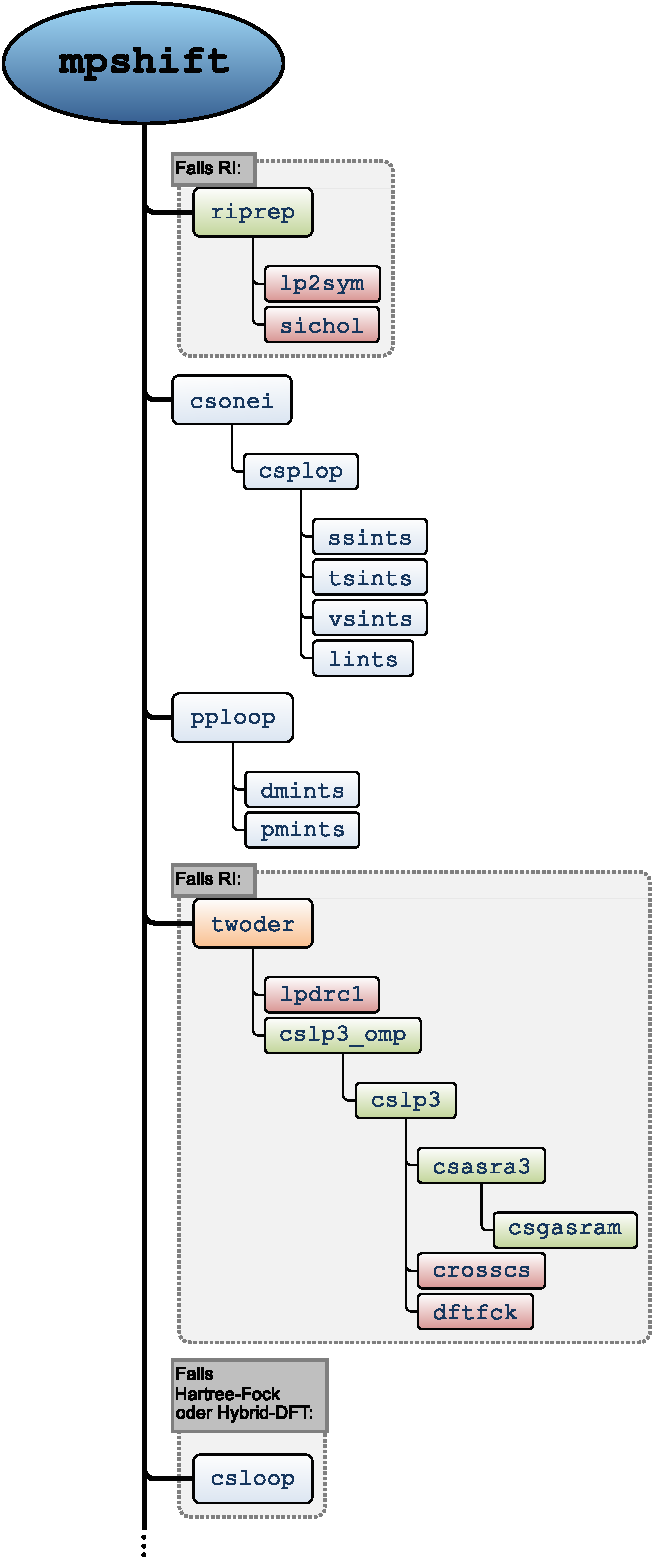
\includegraphics[width=0.55\textwidth]{programmstruktur_ri}
\captionsetup{figurewithin = chapter}
\captionsetup{font=small, labelfont=bf}\caption[\ac{ri}-\textit{J}-Routinen für chemische Abschirmungskonstanten]{Schematische Darstellung der wichtigsten Routinen für die \ac{ri}-\textit{J}-Näherung zur Berechnung chemischer Abschirmungskonstanten im Modul \texttt{mpshift}. Alte Routinen sind in blau, neue Routinen in grün, modifizierte Routinen in orange und unverändert übertragene Routinen in rot dargestellt.}
\label{abb:programmstrukur_ri}
\end{figure}

\section{Die \acs{marij}-Methode für chemische Abschirmungskonstanten}\label{marij}
Eine weitere Beschleunigung bei der Berechnung der Coulombintegrale lässt sich durch die \aclu*{marij-}\mbox{(\acs{marij}-)}\acused{marij}Näherung erreichen. Bei dieser Methode wird der Coulombbeitrag in einen Nahfeld- und einen Fernfeld-Beitrag aufgeteilt. Der Nahfeld-Beitrag wird dabei durch die im vorherigen Abschnitt beschriebene \ac{ri}-Näherung berechnet. Die Berechnung des Fernfeld-Beitrages erfolgt mithilfe einer Multipolentwicklung und ist damit namensgebend für die Methode. Im Vergleich zu konventionellen \ac{ri}-Rechnungen konnte mit der \ac{marij}-Methode eine bis zu 6.5-fache Beschleunigung der Gesamtrechenzeit berichtet werden, ohne dabei einen nennenswerten Verlust an Genauigkeit zu erleiden.\supercite{sierka2003fast}

	\subsection{Theorie}
	Dieser Abschnitt widmet sich der Berechnung des Fernfeld-Beitrages für den Coulombterm und geht auf die Formulierungen von White und Head-Gordon\supercite{white1994derivation} zurück. Die folgende Darstellung folgt Referenz \cite{sierka2003fast}, woraus die wesentlichen Formeln entnommen wurden. 
	
	Zunächst kann der Abstand zweier Elektronen $\vert\vec{r}_1-\vec{r}_2\vert$ durch den Abstand zweier Kerne $R_{\mu\nu}=\vert\vec{R}_\mu-\vec{R}_\nu\vert$ und den entsprechenden Kern-Elektron-Abständen $r_\mu$ und $r_\nu$ ausgedrückt werden,
	\begin{equation}
	\frac{1}{\vert\vec{r}_1-\vec{r}_2\vert}=\frac{1}{\vert\vec{R}_{\mu\nu}-\vec{r}_\mu+\vec{r}_\nu\vert}=\sum_{l=0}^{\infty}\sum_{m=-l}^l O_{lm}(\vec{r}_\mu)\left[\sum_{j=0}^{\infty}\sum_{k=-j}^jB_{jk}^{lm}(\vec{R}_{\mu\nu})O_{jk}(\vec{r}_\nu)\right].
	\end{equation}
	
	Für einen gegebenen Punkt $\vec{r}=(r,\theta,\phi)$ in Kugelkoordinaten sind die Elemente $B_{jk}^{lm}(\vec{r})=M_{l+j,m+k}(\vec{r})$ und $O_{lm}(\vec{r})$ gegeben durch
	\begin{equation}
	O_{lm}(\vec{r})=\frac{r^l}{(l+\vert m\vert)!}P_{lm}(\cos \theta)e^{-\iu m\phi}
	\end{equation}
	
	und 
	\begin{equation}
	M_{l,m}(\vec{r})=\frac{(l-\vert m\vert)!}{r^{l+1}}P_{lm}(\cos \theta)e^{\iu m\phi}
	\end{equation}
	
	mit den entsprechenden Legendre-Polynomen $P_{lm}$. Auf diese Weise lässt sich die Coulombwechselwirkung zweier entfernter Ladungsverteilungen $\rho^O$ und $\rho^R$ entwickeln,
	\begin{equation}\label{eq:marijexpansion}
	\begin{aligned}
	J_{OR}=&\frac{1}{2} \iint\frac{\rho^O(\vec{r}_1)\rho^R(\vec{r}_2)}{\vert\vec{r}_1-\vec{r}_2\vert}\Diff3\vec{r}_1\Diff3\vec{r}_2=\frac{1}{2}\iint\frac{\rho^O(\vec{r}_\mu)\rho^R(\vec{R}_{\mu\nu}+\vec{r}_\nu)}{\vert\vec{R}_{\mu\nu}-\vec{r}_\mu+\vec{r}_\nu\vert}\Diff3\vec{r}_\mu\Diff3\vec{r}_\nu\\
	=&\frac{1}{2}\sum_{l=0}^\infty\sum_{m=-l}^l\mathit{\Omega}_{lm}^O\left[\sum_{j=0}^\infty\sum_{k=-j}^jB_{jk}^{lm}(\vec{R}_{\mu\nu})\mathit{\Omega}_{jk}^P\right]=\frac{1}{2}\sum_{l=0}^\infty\sum_{m=-l}^l\mathit{\Omega}_{lm}^O\mathit{\Xi}_{lm}^P\, .
	\end{aligned}
	\end{equation}
	
	Die $\mathit{\Xi}_{lm}^P$ sind die Koeffizienten einer lokalen Taylor-Entwicklung des durch eine Ladungsverteilung am Punkt $P$ erzeugten Potentials um den Ursprung,
	\begin{equation}
	\mathit{\Xi}_{lm}^P=\sum_{j=0}^\infty\sum_{k=-j}^jB_{jk}^{lm}(\vec{R}_{\mu\nu})\mathit{\Omega}_{jk}^P\, .
	\end{equation}
	
	Die in Gleichung (\ref{eq:marijexpansion}) auftretenden $\mathit{\Omega}_{lm}^O$ und $\mathit{\Omega}_{jk}^P$ sind die Multipolmomente mit ihrem jeweiligen Zentrum am Ort $\vec{O}$ bzw. $\vec{P}$. Im Rahmen der Basissatzentwicklung sind sie gegeben durch
	\begin{equation}\label{eq:multipole}
	\mathit{\Omega}^Q_{lm}=\sum_{\mu,\nu \in Q}D_{\mu\nu}\int\chi_\mu O_{lm}(\vec{r}-\vec{Q})\chi_{\nu}\Diff3 \vec{r}\, .
	\end{equation}
	
	Der Ausdruck auf der rechten Seite von Gleichung (\ref{eq:marijexpansion}) hat den Vorteil, dass sich die Coulombwechselwirkung zweier Ladungsverteilungen nun durch die voneinander unabhängigen Multipolmomente berechnen lässt, da die Information über die gegenseitige Lage der Ladungsverteilungen nur noch in $B_{jk}^{lm}$ steckt. Sind die Multipolmomente einer Ladungsverteilung einmal berechnet, so lassen sich mit ihnen die Coulombwechselwirkungen mit allen anderen Ladungsverteilungen berechnen.\supercite{sierka2003fast}
	 
	\subsection{Implementierung}
Zur Gewährleistung der Eichinvarianz bei der Berechnung chemischer Abschirmungskonstanten mit der \ac{marij}-Methode müssen anstelle gewöhnlicher Basisfunktionen ebenfalls \acp{giao} für Gleichung (\ref{eq:multipole}) verwendet werden. Die Ableitung von Gleichung (\ref{eq:multipole}) nach den Komponenten des Magnetfeldes ist damit gegeben durch

	\begin{equation}\label{eq:multipoledb}
	\begin{aligned}
	\left.\frac{\partial \Omega^Q_{lm}}{\partial B_\beta}\right\vert_{\vec{B}=0}=&\Omega^{Q,B_\beta}_{lm}=\frac{\iu}{2c}\sum_{\mu,\nu \in Q}D_{\mu\nu}\int\left(\vec{R}_{\mu\nu}\times\vec{r}\right)_\beta\chi_\mu^{\vec{B}=0} O_{lm}(\vec{r}-\vec{Q})\chi_{\nu}^{\vec{B}=0}\Diff3 \vec{r}\\
	=&\frac{\iu}{2c}\sum_{\mu,\nu \in Q}\left(\vec{R}_{\mu}\times\vec{R}_{\nu}\right)_\beta D_{\mu\nu}\int\chi_\mu^{\vec{B}=0}O_{lm}(\vec{r}-\vec{Q})\chi_{\nu}^{\vec{B}=0}\Diff3\vec{r}\\
	&+\frac{\iu}{2c}\sum_{\mu,\nu \in Q}D_{\mu\nu}\left(\vec{R}_{\mu\nu}\times\int\vec{r}_{\mu}\chi_\mu^{\vec{B}=0}O_{lm}(\vec{r}-\vec{Q})\chi_{\nu}^{\vec{B}=0}\Diff3\vec{r}\right)_\beta \, .
	\end{aligned}
	\end{equation}
	Dieser Ausdruck wird schließlich in Gleichung (\ref{eq:marijexpansion}) eingesetzt, woraus der durch Multipolmomente genäherte Beitrag für den Coulombterm resultiert. Zur Berücksichtigung der \ac{marij}-Beiträge wurde die Routine \texttt{twoder} um den Aufruf der modifizierten Routine \texttt{fmmlpdrc2} erweitert. Deren Funktion sowie von ihr aufgerufener Unterroutinen sind im Folgenden erläutert. Eine schematische Darstellung der wichtigsten Routinen zur Berechnung der \ac{marij}-Beiträge für chemische Abschirmungskonstanten ist in Abbildung \ref{abb:programmstrukur_marij} gezeigt.
	\begin{itemize}[leftmargin=70pt]
	\item[\texttt{initmulopt}:] Initialisierung für die Multipolnäherung. Sofern in der \texttt{control}-Datei Optionen spezifiziert wurden, werden sie an dieser Stelle eingelesen und ersetzen die Standardwerte.
	\item[\texttt{auxmaxmom}:] Bestimmung der maximalen Drehimpulsquantenzahl in den Auxiliarbasisfunktionen.
	\item[\texttt{extdef}:] Bestimmung der Multipolmomentzentren für das Schalenpaar zweier Basisfunktionen.
	\item[\texttt{fmmlpdrc1}:] Berechnung des Fernfeld-Beitrages zu $\Gamma_Q$ in der Multipolnäherung.
	\item[\texttt{fmmlpdrc2}:] Berechnung des Fernfeld-Beitrages zur Coulombmatrix in der Multipolnäherung.
	\item[\texttt{auxmom2}:] Berechnung der Multipolmomente für die Auxiliarbasisfunktionen und anschließende Kontraktion mit den Elementen von $\Gamma_P$.
	\item[\texttt{mktayaux}:] Berechnung der Koeffizienten der lokalen Taylor-Entwicklung für die Auxiliarschalen.
	\item[\texttt{csmunumom}:] Für die Berechnung von chemischen Abschirmungskonstanten modifizierte Version von \texttt{munumom2}. Hier erfolgt die Berechnung des Fernfeld-Beitrages zur Coulombmatrix in der Multipolnäherung durch Kontraktion der Taylor-Koeffizienten der Auxiliarbasisfunktionen mit den Multipolmomenten der Schalenpaare zweier Basisfunktionen.
	\item[\texttt{cssphmom}:] Für die Berechnung von chemischen Abschirmungskonstanten modifizierte Version von \texttt{sphmom}. Berechnung der Multipolintegrale.
	\item[\texttt{lsprim}:] Berechnung der Multipolintegrale für die primitiven Basisfunktionen $\int l_0 O_{lm} l_0\Diff3\vec{r}$ bis $\int l_0 O_{lm} l_{ij+2} \Diff3\vec{r}$ (vertikale Rekursion), wobei $l_{ij+2}$ die Summe der Drehimpulsquantenzahlen der $i$- und $j$-Schale $+2$ ist.
	\item[\texttt{cshorsph}:] Für die Berechnung von chemischen Abschirmungskonstanten modifizierte Version von \texttt{horsph}. Berechnung aller benötigten Integrale  $\int l_i O_{lm} l_j\Diff3\vec{r}$ durch horizontale Rekursion.
	\item[\texttt{cscross}:] Berechnung der Kreuzproduktterme aus den einzelnen Integralen, um den vollständigen Beitrag aus der Multipolnäherung für die Coulombmatrix zu erhalten.
	\end{itemize}
	
\begin{figure}[ht!]
\centering
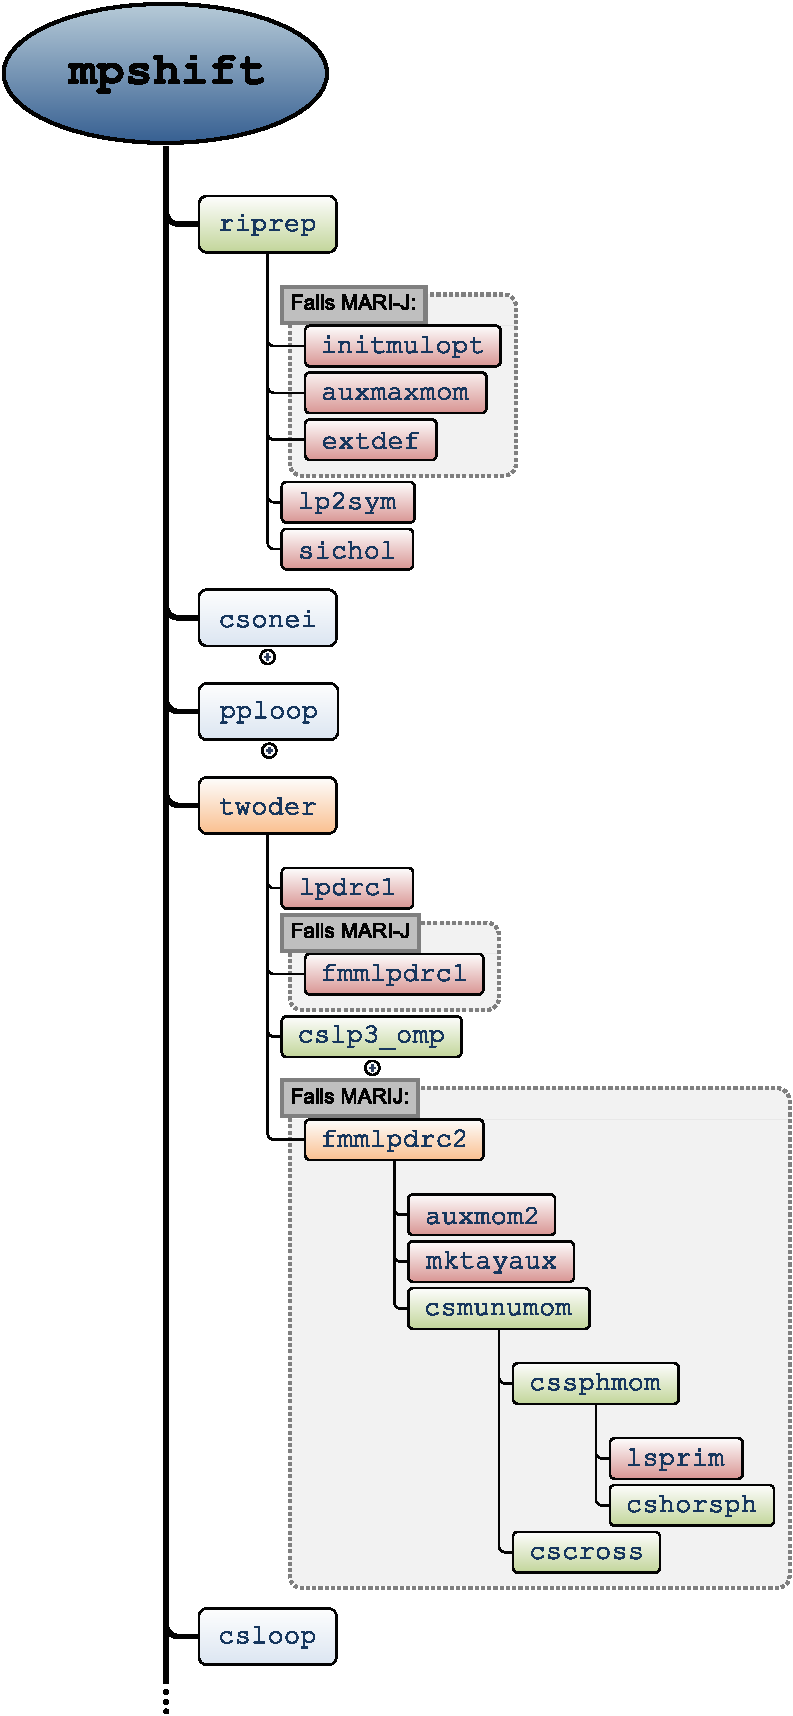
\includegraphics[width=0.6\textwidth]{programmstruktur_marij}
\captionsetup{figurewithin = chapter}
\captionsetup{font=small, labelfont=bf}\caption[\ac{marij}-Routinen für chemische Abschirmungskonstanten]{Schematische Darstellung der wichtigsten Routinen für die \ac{marij}-Näherung zur Berechnung chemischer Abschirmungskonstanten im Modul \texttt{mpshift}. Alte Routinen sind in blau, neue Routinen in grün, modifizierte Routinen in orange und unverändert übertragene Routinen in rot dargestellt.}
\label{abb:programmstrukur_marij}
\end{figure}



\section{Parallelisierung und Programmoptimierungen}\label{paraopt}
Bei bestimmten Verbindungen kann es von Interesse sein, die chemischen Abschirmungskonstanten nur für eine Auswahl an Atomen zu berechnen. Beispielsweise wenn nur eine bestimmte Atomsorte von Interesse ist oder lediglich die chemische Verschiebung in einem bestimmten Bereich untersucht werden soll. In diesen Fällen kann es zu einer Rechenzeitersparnis kommen wenn nur Beiträge für ausgewählte Atome oder Atomsorten berechnet werden. Aus diesem Grund wurde das Modul \texttt{mpshift} um die Möglichkeit ergänzt, eine Auswahl der zu berechnenden Atome zu treffen. Im Programmcode selbst ist dies auf die einfache Weise realisiert, dass die Ableitungen nach den Komponenten der Kernmomente sowie der gesamte Abschirmungstensor nur für die ausgewählten Atome berechnet werden. Dies kann durch Hinzufügen des Keywords \texttt{\$nucsel} in der \texttt{control}-Datei erreicht werden. Durch die Eingabe von \texttt{\$nucsel "N","Fe"} lassen sich beispielsweise die chemischen Abschirmungskonstanten für alle Sickstoff- und Eisenatome im Molekül berechnen. Mit \texttt{\$nucsel 1,3,5-8} erfolgt die Berechnung für die Atome Nummer 1,3,5-8 in der \texttt{coord}-Datei. Sind in größeren organischen Molekülen, welche von Wasserstoff- und Kohlenstoffatomen dominiert werden, alle $^1$H- oder $^{13}$C-Abschirmungskonstanten von Interesse, so liefert dieses vorgehen in der Regel jedoch kaum eine Zeitersparnis und es können direkt die Abschirmungskonstanten aller Atome berechnet werden. Umgekehrt lassen sich auf diese Weise auch Elemente aus der Rechnung ausschließen, welche ohnehin nicht von Interesse sind, aber gegebenenfalls für ein schlechtes Konvergenzverhalten während der \ac{cphf}-Iterationen sorgen.

\bigskip
Das bisherige, standardmäßige Auswählen des ersten Atoms aus der \texttt{coord}-Datei für den Konvergenztest bei den \ac{cphf}-Iterationen lässt sich ebenfalls optimieren. In der Praxis hat sich herausgestellt, dass insbesondere für schwere Elemente mehr Iterationen benötigt werden, bis die Konvergenz erreicht wird. Dies liegt auch daran, dass die Absolutwerte für die chemischen Abschirmungskonstanten dieser Elemente mit zunehmender Ordnungszahl steigen. Die Konvergenz wurde aber standardmäßig auf eine Änderung von weniger als \unit[$1\times 10^{-2}$]{ppm} gesetzt, unabhängig vom jeweiligen Element. Hierfür wurde ein Faktor eingeführt, welcher die Ordnungszahl des entsprechenden Elements berücksichtigt und die Konvergenz für Elemente mit hoher Ordnungszahl ein wenig lockert. Weiterhin hat sich herausgestellt, dass Atome die weit vom Koordinatenursprung entfernt sind, ebenfalls länger bis zur Konvergenz benötigen. Daher erfolgt die Atomauswahl für den Konvergenztest bei den \ac{cphf}-Iterationen dermaßen, dass zunächst das schwerste Element im Molekül gesucht wird. Sollte es davon mehrere geben, dann wird daraus das Atom ausgewählt, welches am weitesten vom Ursprung entfernt liegt. Dieses Vorgehen hat den Vorteil, dass in der Regel nur in den letzten beiden Iterationen die chemischen Abschirmungskonstanten für alle Atome berechnet werden müssen, um zu überprüfen, ob alle Atome bereits konvergiert sind. Da der kritischste Fall zu diesem Zeitpunkt in der Regel bereits zur Konvergenz gebracht werden konnte, ist dies üblicherweise gegeben.

\bigskip
Wird die \ac{ri}- bzw. \ac{marij}-Methode in einer Hartree-Fock- bzw. Hybrid-\ac{dft}-Rechnung verwendet, so wird der Austauschbeitrag unabhängig vom Coulombbeitrag berechnet. Für Ersteren kann jedoch eine effizientere Integralabschätzung\supercite{ochsenfeld1998linear} angewendet werden als für den Coulombbeitrag. Aus diesem Grund wurden die Integralabschätzungen aus der Routine \texttt{shloop\_k}, welche die ungestörten Austauschmatrixelemente während des \ac{scf}-Verfahrens oder während der \ac{cphf}-Iterationen berechnet, in die Routine \texttt{csloop} übertragen. Auf diese Weise kann die Berechnung kleiner bzw. später verschwindender Matrixelemente vermieden werden. Des Weiteren wurde die Routine \texttt{shloop}, welche in der Routine \texttt{cpscf} zur Berechnung der ungestörten Vierzentren-Zweielektronen-Integrale gerufen wird, durch die Routine \texttt{hf\_k} ersetzt. Das ist darin begründet, dass die Spur des Produkts der symmetrischen Coulombmatrix und der antisymmetrischen Dichtematrix verschwindet, wodurch der Coulombbeitrag an dieser Stelle nicht mehr benötigt wird. Lediglich der Austauschbeitrag muss berechnet werden, wofür die Routine \texttt{hf\_k} optimiert ist. Beim iterativen Lösen der \ac{cphf}-Gleichungen kann zusätzlich durch das Bilden von Differenzdichten (aus der aktuellen und vorherigen Iteration) profitiert werden. 

\bigskip
Neben einer effizienten Programmierung und dem Einführen von Näherungen, wie beispielsweise bei der \ac{ri}- bzw. \ac{marij}-Methode, kann die Laufzeit einer Rechnung auch durch eine Parallelisierung des Programmcodes reduziert werden. Dies ist insofern von besonderer Bedeutung, dass heutige Computer immer mehr CPUs zur Verfügung haben. Selbst in gewöhnlichen Desktop-PCs oder Notebooks finden sich häufig mindestens 4 CPUs. Aus diesem Grund wurden die zeitaufwändigsten Routinen im \texttt{mpshift}-Modul mit OpenMP\supercite{dagum1998openmp} in Zusammenarbeit mit Fabian Mack parallelisiert. Im Einzelnen betrifft dies die Routinen \texttt{csloop}, \texttt{cslp3\_omp}, \texttt{csplop}, \texttt{shloop\_k}, \texttt{p3loop} und \texttt{pploop}. Die Routinen \texttt{csplop}, \texttt{p3loop} und \texttt{pploop} besitzen üblicherweise folgende grundlegende Schleifenstruktur:
\vfill
\newpage
\texttt{do i=1,N$_{\texttt{Schal}}$}\\ 
\null\quad\texttt{do j=1,N$_{\texttt{Schal}}$}\\ 
\null\quad\quad\texttt{do $\mu$=1,N$_{\texttt{Prim BF}}$}\\ 
\null\quad\quad\quad\texttt{do $\nu$=1,N$_{\texttt{Prim BF}}$}\\
\null\quad\quad\quad\quad \texttt{Auszuführender Programmcode}\\ 
\null\quad\quad\quad\texttt{end do}\\ 
\null\quad\quad\texttt{end do}\\ 
\null\quad\texttt{end do}\\ 
\texttt{end do}\\
\\
Die äußeren beiden Schleifen laufen dabei über alle Schalen \texttt{N}$_{\texttt{Schal}}$ und die beiden inneren Schleifen laufen über die primitiven Basisfunktionen \texttt{N}$_{\texttt{Prim BF}}$. Für die Routine \texttt{cslp3\_omp} kommt jeweils eine weitere Schleife für die Auxiliarschale und die primitiven Auxiliarbasisfunktionen hinzu. Bei den Vierzentren-Routinen \texttt{csplop} und \texttt{shloop\_k} sind es jeweils zwei weitere Schleifen für die Schalen und die primitiven Basisfunktionen. Bei der Parallelisierung wurde nun in der Regel so vorgegangen, dass die äußerste Schleife über die Schale parallelisiert wurde:\\
\\
\texttt{\$OMP PARALLEL}\\
\texttt{\$OMP DO SCHEDULE (DYNAMIC)}\\
\texttt{do i=1,N$_{\texttt{Schal}}$}\\ 
\null\quad\texttt{do j=1,N$_{\texttt{Schal}}$}\\ 
\null\quad\quad\texttt{do $\mu$=1,N$_{\texttt{Prim BF}}$}\\ 
\null\quad\quad\quad\texttt{do $\nu$=1,N$_{\texttt{Prim BF}}$}\\
\null\quad\quad\quad\quad \texttt{Auszuführender Programmcode}\\ 
\null\quad\quad\quad\texttt{end do}\\ 
\null\quad\quad\texttt{end do}\\ 
\null\quad\texttt{end do}\\ 
\texttt{end do}\\
\texttt{\$OMP END DO}\\
\texttt{\$OMP END PARALLEL}\\
\\
